\subsection{Uncertainties in gas chemistry}
Accurate simulation of soot and carbon black formation remains a major challenge due to the compounded uncertainties in both gas-phase chemistry and particle dynamics. One of the central difficulties lies in the limited quantitative understanding of soot inception and surface growth mechanisms. The pathways and rate constants for elementary reactions governing PAH dimerization, radical interactions, and surface reactions are not well established. As a result, any sub-model used to describe soot inception and surface growth introduces significant uncertainties when coupling gas-phase chemistry with particle dynamics.

These uncertainties are built upon those already present in detailed chemical kinetic mechanisms, particularly in predicting intermediate species such as acetylene ($\mathrm{C_2H_2}$) and polycyclic aromatic hydrocarbons (PAHs). Prior studies have shown that the predicted concentrations of large PAHs can vary by orders of magnitude depending on the chosen reaction mechanism. Consequently, soot models inherit uncertainty from two sources: (i) the reaction mechanism used to describe fuel pyrolysis and oxidation, and (ii) the choice of inception and surface growth models and parameters. The cumulative effect significantly complicates efforts to produce reliable predictions of soot mass and morphology.

In contrast, particle dynamics models introduce a relatively low uncertainty when provided with accurate estimates of carbon flux from inception and surface growth. These models, particularly when well-validated, are capable of accurately predicting key particle properties such as volume fraction, size distribution, and agglomerate morphology. This highlights the importance of coupling between gas-phase chemistry and soot formation models: the reliability of soot and carbon black simulations hinges less on the particle dynamics approach itself and more on the accuracy of upstream chemical kinetics, inception and surface growth fluxes.

To illustrate the impact of chemical mechanism selection on precursor formation, a series of simulations\footnote{\href{https://github.com/mohammadadib-cu/omnisoot-cv/tree/main/examples/pressure/mechanism_comparison}{https://github.com/mohammadadib-cu/omnisoot-cv/tree/main/examples/pressure/mechanism\_comparison}} were performed using the CPR model of omnisoot (with soot formation disabled) for the pyrolysis of $5\%$ $\mathrm{CH_4}$-Ar mixture at $\mathrm{T_5}=$2200 K. Seven widely used mechanisms were evaluated: ABF~\citep{appel2000kinetic}, Caltech~\citep{blanquart2009chemical}, KAUST~\citep{wang2013pah}, CRECK~\citep{saggese2015kinetic}, ITV~\citep{hellmuth2024role}, NUIG~\citep{zhu2023wide}, and FFCM2~\citep{ZDV2023}. These mechanisms have varying degrees of complexity and validation histories, particularly in high-temperature pyrolysis environments


The comparison focuses on the predicted Carbon Mass Fraction (CMF) of species involved in soot formation. Here, CMF is defined as the mass of carbon in a given species normalized by the total carbon mass in the gas mixture. Initially, the CMF of methane is equal to 1, indicating that all carbon is stored in $\mathrm{CH_4}$ at $t = 0$ in the studied shock tube. %It should be noted that the CRECK mechanism used in this work does not include ``BIN" species, except for BIN1.


Figure~\ref{fig:CH4_C2H4_A2R5_chem} shows the variability in the predicted CMF of $\mathrm{CH_4}$, $\mathrm{C_2H_2}$, and A2R5 across different reaction mechanisms. The CMF of $\mathrm{CH_4}$ serves as a useful indicator of carbon flux from the fuel to intermediate species. $\mathrm{C_2H_2}$ is the most abundant hydrocarbon during pyrolysis and plays a key role in the HACA mechanism for PAH growth beyond benzene, as well as in surface growth of soot. A2R5 has been identified as important for soot inception due to its propensity for radical interaction and molecular stacking~\citep{martin2019reactivity}.

As shown in the inset of Figure~\ref{fig:CH4_C2H4_A2R5_chem}a, the CRECK mechanism predicts the highest $\mathrm{CH_4}$ conversion up to 1 ms, but this trend reverses at longer residence times, where KAUST predicts the lowest CMF. ABF, FFCM2 and NUIG underpredict the methane conversion rate by nearly 10\% of the initial carbon compared to the other mechanisms. As expected, the majority (60–80\%) of the initial carbon is converted to $\mathrm{C_2H_2}$ by the end of the simulation. In the inset of Figure~\ref{fig:CH4_C2H4_A2R5_chem}b, all mechanisms direct more carbon toward $\mathrm{C_2H_2}$ by 5 ms. CRECK predicts the highest $\mathrm{C_2H_2}$ CMF up to 3.5 ms, after which NUIG and FFCM2 gives the largest $\mathrm{C_2H_2}$ CMF. This is attributed to FFCM2 and NUIG’s lack of aromatic and large hydrocarbon species, so it does not account for the conversion of $\mathrm{C_2H_2}$ to PAHs.

The relative difference between the mechanisms is most pronounced for A2R5, spanning over an order of magnitude between ABF and KAUST. This aligns with previous findings that the uncertainty in the predicted concentration of gas-phase species increases with molecular size~\cite{wang2023systematic}. This highlights the escalating uncertainty with increasing molecular size of PAHs and reinforces that any inception model built on these predictions inherits and amplifies such uncertainties.
 
\begin{figure}[H]
	\centering
	\begin{subfigure}[t]{0.31\textwidth}
		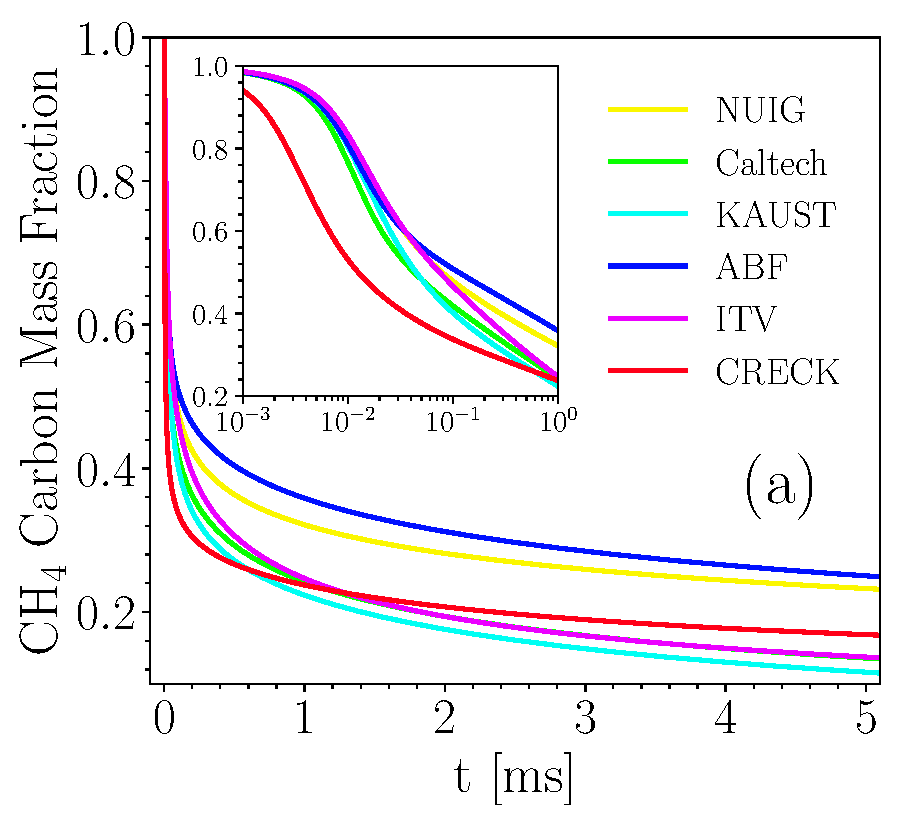
\includegraphics[width=1\textwidth]{Figures/Results/chemistry/CH4.pdf}
	\end{subfigure}
	\begin{subfigure}[t]{0.31\textwidth}
		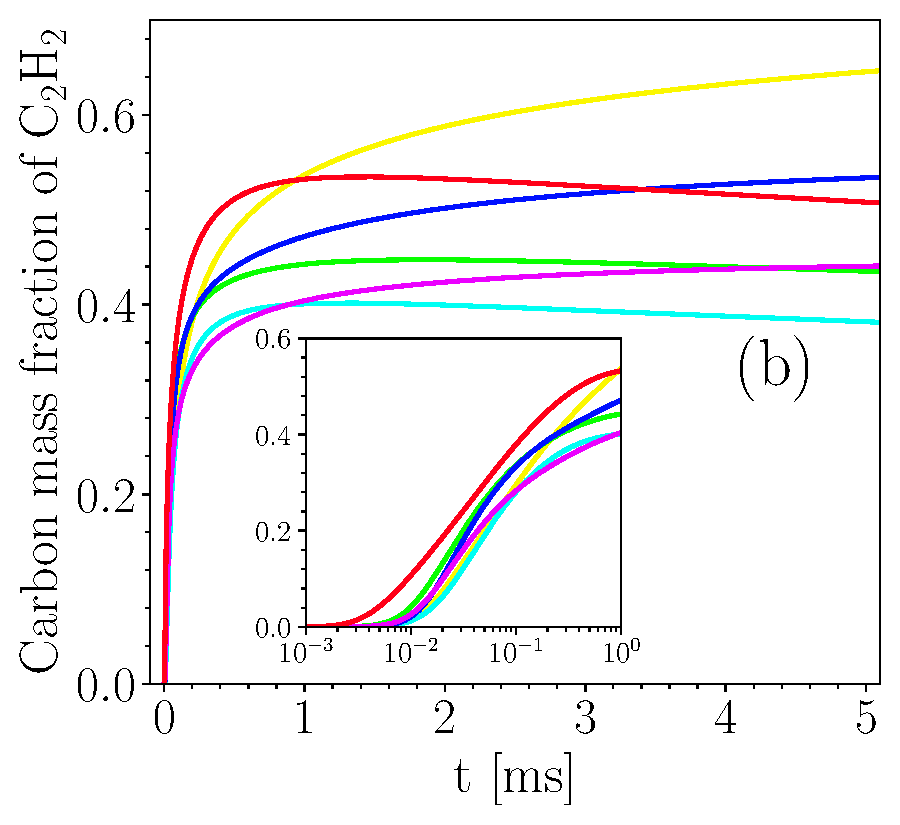
\includegraphics[width=1\textwidth]{Figures/Results/chemistry/C2H2.pdf}
	\end{subfigure}
	\begin{subfigure}[t]{0.31\textwidth}
		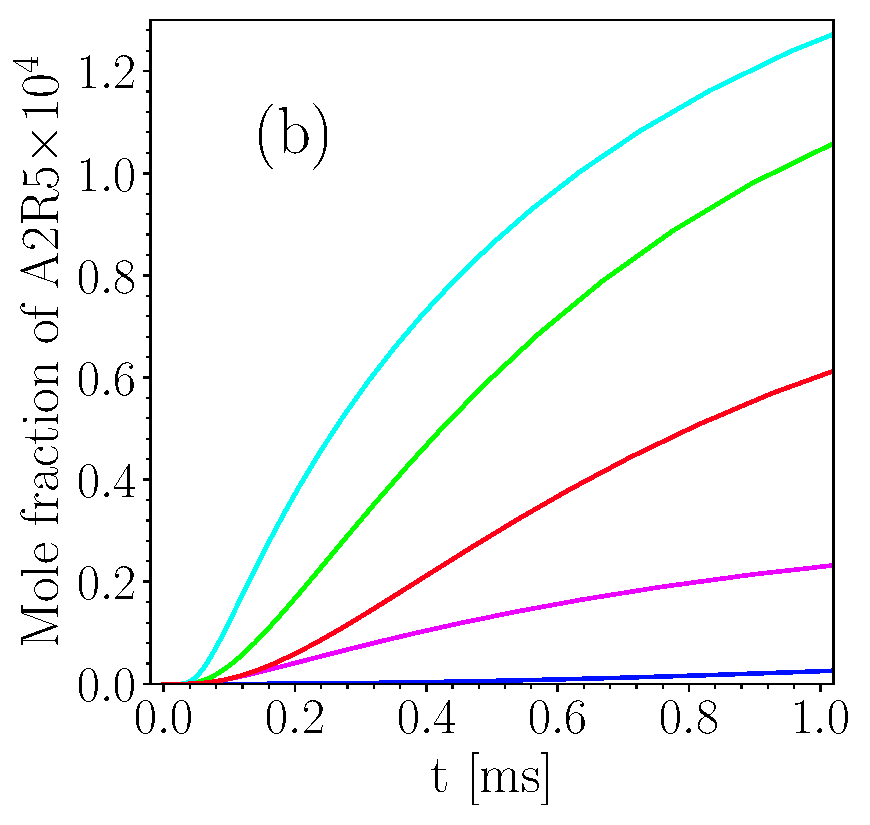
\includegraphics[width=1\textwidth]{Figures/Results/chemistry/A2R5.pdf}
	\end{subfigure}
	\caption{The carbon mass fraction of $\mathrm{CH_4}$ (a), $\mathrm{C_2H_2}$ (b), and A2R5 (c) during pyrolysis of 10\%~$\mathrm{CH_4}$-Ar predicted using different reaction mechanisms. The insets provide a zoomed-in view of the early-time behavior}
	\label{fig:CH4_C2H4_A2R5_chem} 
\end{figure}

The uncertainties in the precursors chemistry coupled with the poorly constrained pathways for soot inception and surface growth results in the compounded uncertainty that changes soot yield, particle number concentration and characteristic diameters by orders of magnitude depending on the temperature, pressure and fuel composition in studied targets. For these reasons, we avoid evaluating inception models based on their absolute accuracy. Instead, we selected reaction mechanisms that provide enough carbon flux to soot precursors (listed in Table~\ref{tab:precursors_list}) that allows adjusting inception and surface growth flux using the corresponding factors ($\eta_{inc}$ and $\eta_{ads}$) to match simulated soot volume fraction, particle size (e.g., $d_p$ or $d_m$), or PSD. Among the mechanisms tested, only the Caltech, KAUST, and ITV models met these criteria. The ITV mechanism, however, was not used in this study due to its large size (759 species and 7582 reactions), which makes it too computationally expensive for parametric studies.


It should be noted that the calibration process does not resolve the mechanistic uncertainties of soot formation. it allows the model to back-calculate effective carbon fluxes from the gas phase into the particle phase that are consistent with measured soot characteristics. When combined with a well-validated particle dynamics model, this approach provides a robust means of quantifying the net impact of chemistry and bridging the uncertainty gap between molecular-scale kinetics and macroscale soot morphology.
%
%\begin{figure}[H]
%	\centering
%	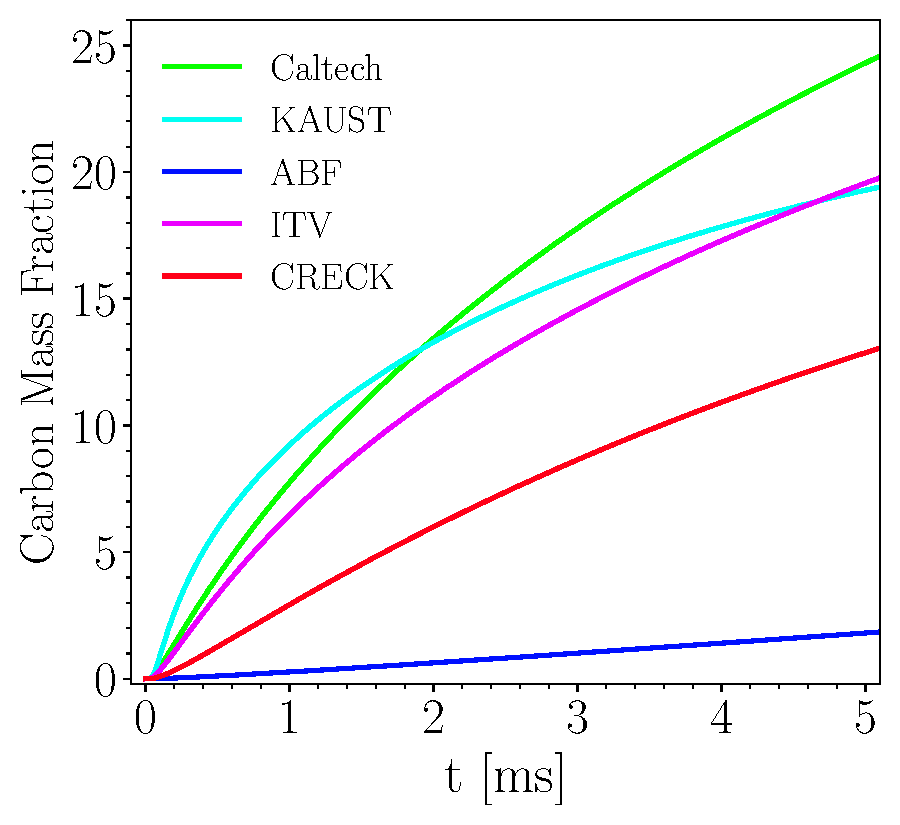
\includegraphics[width=0.32\textwidth]{Figures/Results/chemistry/med_hydrocarbons.pdf}
%	\caption{The carbon mass fraction of $\mathrm{C_{10}}$ to  $\mathrm{C_{18}}$ during pyrolysis of 10\%~$\mathrm{CH_4}$-Ar predicted using different reaction mechanisms}
%	\label{fig:PAHs_chem} 
%\end{figure}